\documentclass[a4paper,10pt]{article} % добавить leqno в [] для нумерации слева
\usepackage[a4paper,top=1.3cm,bottom=2cm,left=1.5cm,right=1.5cm,marginparwidth=0.70cm]{geometry}

\usepackage[warn]{mathtext}
\usepackage[T2A]{fontenc}
\usepackage[utf8]{inputenc} 
\usepackage[english, russian]{babel}

\usepackage{ upgreek }
\usepackage[table,xcdraw]{xcolor}

\usepackage{indentfirst} %tabutation

\usepackage{amsmath, amsfonts, amssymb, amsthm, mathtools, mathtext} 

\usepackage{graphicx}

\usepackage{wrapfig}
\usepackage{tabularx}

\usepackage{graphicx}%Вставка картинок правильная
\usepackage{float}%"Плавающие" картинки
\usepackage{wrapfig}% Обтекание фигур (таблиц, картинок и прочего)

%%% Дополнительная работа с математикой
\usepackage{amsmath,amsfonts,amssymb,amsthm,mathtools} % AMS





%%% Заголовок
\author{Устюжанина Мария Алексеевна}
\title{Лабораторная работа №1.2.3
Отчет о выполнении лабораторной работы 1.2.
}
\date{\today}

\begin{document}

\begin{titlepage}
	\begin{center}
		{\large МОСКОВСКИЙ ФИЗИКО-ТЕХНИЧЕСКИЙ ИНСТИТУТ (НАЦИОНАЛЬНЫЙ ИССЛЕДОВАТЕЛЬСКИЙ УНИВЕРСИТЕТ)}
	\end{center}
	\begin{center}
		{\large Физтех-школа радиотехники и компьютерных технологий}
	\end{center}
	
	
	\vspace{4cm}
	{\huge
		\begin{center}
			{\bf Лабораторная работа № 2.4.1}\\
			 Определение теплоты испарения жидкости.
		\end{center}
	}
	\vspace{3cm}
	\begin{flushright}
		{\LARGE Авторы:\\ Устюжанина Мария Алексеевна,

		Федорищева Анастасия Анатольевна, 

		Романов Александр Викторович, 

		Пархоцевич Иван Николаевич\\
			\vspace{0.3cm}
			Б01-107}
	\end{flushright}
	\vspace{4.5 cm}
	\begin{center}
		Долгопрудный 2022

	\vspace{1 cm}

		 *В данном исследовании был изучен жизненно важно очень необходимый, волнующий всех вопрос. Надеемся, что наши читатели будут крайне благодарны нам за столь ценные выводы, которые они сделают после прочтения. 
		 Целью нашей работы является вдохновение читателей!

	\end{center}
\end{titlepage}

\section{Введение}

Вопросам, связанным с исследованием испарения жидкости, было посвящено большое количество исследований, что связано с практической важностью этого направления. 

Испарение жидкости играет ведущую роль в отраслях промышленности. Именно поэтому продолжение исследований особенностей его протекания является актуальным и по сей день как с теоретической, так и с практической точки зрения.

\textbf{Цель работы:}

1) Измерение давления насыщенного пара жидкости при разной температуре; 

2) Вычисление по полученным данным
теплоты испарения с помощью уравнения Клапейрона–Клаузиуса.

\textbf{Используемое оборудование:}

Термостат; герметический сосуд, заполненный исследуемой жидкостью; отсчетный микроскоп.

\section{Основная часть}

Одно и то же вещество при одних и тех же температуре и давлении может находиться в газообразном, жидком и твердом состояниях, причем эти состояния (фазы) могут существовать одновременно, находясь в контакте друг с другом.
 Эти состояния отличаются своими физическими свойствами. Переход вещества из одной фазы в другую называется фазовым переходом или фазовым превращением. Испарение — переход жидкости в пар, являются примером фазовых переходов. 

В уравнении Ван-дер-Ваальса жидкость может находиться в равновесии со своим паром. Это равновесие с паром, который в таком случае называется насыщенным паром, устанавливается само собой, если жидкость находится в закрытом сосуде.
Процесс установления равновесия сводится к тому, что с поверхности жидкости вылетает часть молекул, образуя над жидкостью пар. Для выхода из жидкости испаряющиеся молекулы должны преодолеть силы притяжения со стороны оставшихся молекул, т. е. совершить работу против этих сил. Кроме того, должна быть совершена работа против внешнего давления р уже
образовавшегося пара, равная $p\Delta V$, где $\Delta V$ —изменение объема,
занимаемого данным количеством молекул при переходе из жидкости в пар. Вся эта работа может быть совершена только за счет кинетической энергии теплового движения молекул. Очевидно, что не все молекулы способны совершить эту работу, а только те из них, которые обладают достаточной для этого кинетической энергией. Поэтому переход части молекул в пар приводит к обеднению жидкости быстрыми молекулами,т. е. к ее охлаждению.

Давление насыщенного пара какого-либо вещества зависит от температуры и не зависит от объема пара, а также от давления других газообразных примесей, если они трудно растворимы в данной жидкости или в данном твердом теле.

Для вывода соотношения между температурой и давлением насыщенного пара жидкости обычно рассматривают равновесный переход одного моля вещества из одной фазы (1) в дpyгyю (2) при постоянных давлении и температуре. Изобарные потенциалы ($G_i$) единицы массы чистого вещества в двух фазах однокомпонентной системы, находящихся в равновесии, при условии что
число молей компонента в жидкой и паровой фазах равны единице, равны между собой

\[G_1 = G_2\]
\[dG_1 = dG_2\]

Уравнение в дифференциальной форме для  изобарных потенциалов для одного моля в фазах 1 и 2 принимает следующий вид:

\[dG_1 = V_1dp - S_1dT\]
\[dG_2 = V_2dp - S_2dT\]

Вычитая нижнее уравнение из верхнего, получим:
\[dG_2 - dG_1 = (V_2-V_1)dp - (S_2-S_1)dT \]

Следовательно, $(V_2-V_1)dp - (S_2 - S_1)dT = 0$.
Получим уравнение:

\[\frac{dp}{dT} = \frac{S_2 - S_1}{V_2-V_1}\]

Известно, что:

\[S_2 - S_1 = \frac{L}{T,}\]

где L - теплота испарения жидкости.

В уравнении Ван-дер-Ваальса:
\[(P+\frac{a}{V^2})(V-b) = RT\]

принебрежем величинами $b$ и $\frac{a}{V^2}$. Тогда получим: 

\[V = \frac{RT}{P}\]

В итоге для удельной теплоты испарения: 
\[L = \frac{RT^2}{P}\frac{dP}{dT} = -R\frac{d(ln(P))}{d(1/T)}\]



Применяемый нами диагностический метод является классическим и описан в источнике Гладун A.Д. Лабараторный практикум по общей физики. Т.I. Термодинамика и молекулярная физика. стр 234-235.



\medskip

\textbf{Экспериментальная установка.}
Установка включает термостат A, экспериментальный прибор B и отсчетный микроскоп C. Экспериментальный прибор B представляет собой емкость 12, заполненную водой. В нее погружен запаянный прибор 13 с исследуемой жидкостью 14. Перед заполнением исследуемой жидкости воздух
из запаянного прибора был удален, так что над жидкостью находится только её насыщенный пар.
Давление пара определяется по ртутному манометру 15, соединенному с емкостью 13.

\begin{figure}[h]
	\center{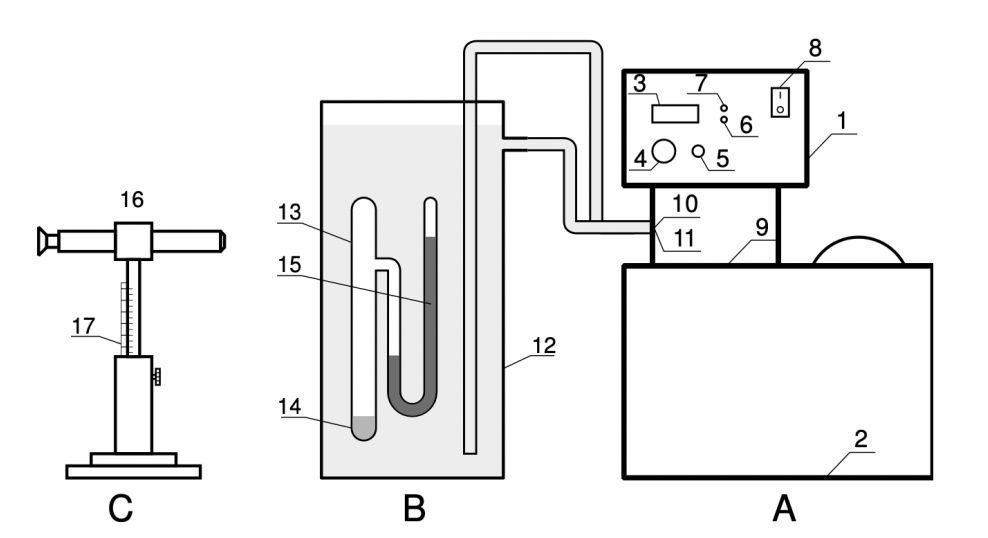
\includegraphics[scale=0.8]{Picture1}}
	\caption{Схема установки для определения теплоты испарения}
\end{figure}

	


\section{Заключение}
	\begin{enumerate}
		\item Все получилось хорошо.
		\item Все живы.
	\end{enumerate}

\section{Список литературы}
	\begin{enumerate}
		\item Сивухин Д.В. Общий курс физики. Т. II. Термодинамика и молекулярная физика.
		\item Гладун A.Д. Лабараторный практикум по общей физики. Т.I. Термодинамика и молекулярная физика.
		\item https://cyberleninka.ru/article/n/issledovanie-temperaturnoy-zavisimosti-skorosti-ispareniya-zhidkostey-so-svobodnoy-poverhnosti-i-skorosti-kipeniya-zhidkosti-na/viewer
		\item https://www.gubkin.ru/faculty/chemical_and_environmental/chairs_and_departments/physical_and_colloid_chemistry/files/fazovoye_ravnovesiye.pdf
	\end{enumerate}


\end{document}